
\documentclass[journal]{IEEEtran}

\usepackage[utf8]{inputenc}
\usepackage[version=3]{mhchem} % Package for chemical equation typesetting
\usepackage{siunitx} % Provides the \SI{}{} and \si{} command for typesetting SI units
\usepackage{graphicx} % Required for the inclusion of images
\usepackage{natbib} % Required to change bibliography style to APA
\usepackage{amsmath} % Required for some math elements 

%grafo
\usepackage{pgf}
\usepackage{tikz}
\usetikzlibrary{arrows,automata}
\usepackage{verbatim}
\usepackage{float}
\usepackage[portuguese]{babel} % English language/hyphenation
\usepackage{subcaption} 
\usepackage{multirow}
\usepackage{setspace}
\usepackage{hyperref}

% correct bad hyphenation here
\hyphenation{op-tical net-works semi-conduc-tor}


\begin{document}

\title{Reconhecimento de Padrões\\ Trabalho Final}

\author{Gian Maurício Fritsche}

\maketitle

\IEEEpeerreviewmaketitle

\section{Descrição do trabalho}

Para a realização deste trabalho foi utilizada a base de imagens SIMPSONS\footnote{\url{http://www.inf.ufpr.br/lesoliveira/padroes/simpsons.zip}}.
O objetivo é construir um sistema de reconhecimento de padrões que discriMínimoe as cinco classes (representando os cinco personagens principais: Bart, Homer, Lisa, Maggie e Marge).

\begin{figure}[!htb]
    \centering
    \begin{subfigure}[b]{0.15\textwidth}
        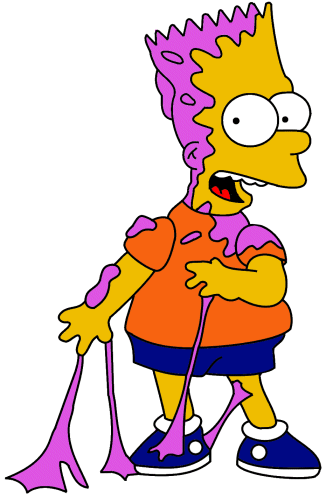
\includegraphics[width=\textwidth]{bart001}
        \caption{Bart}
        \label{fig:bart}
    \end{subfigure}
    ~ %add desired spacing between images, e. g. ~, \quad, \qquad, \hfill etc. 
      %(or a blank line to force the subfigure onto a new line)
    \begin{subfigure}[b]{0.15\textwidth}
        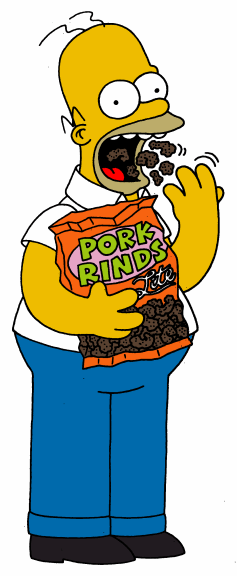
\includegraphics[width=\textwidth]{homer001}
        \caption{Homer}
        \label{fig:homer}
    \end{subfigure}
    ~ %add desired spacing between images, e. g. ~, \quad, \qquad, \hfill etc. 
    %(or a blank line to force the subfigure onto a new line)
    \begin{subfigure}[b]{0.15\textwidth}
        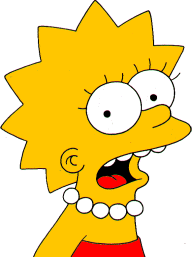
\includegraphics[width=\textwidth]{lisa001}
        \caption{Lisa}
        \label{fig:lisa}
    \end{subfigure}
    ~ %add desired spacing between images, e. g. ~, \quad, \qquad, \hfill etc. 
    %(or a blank line to force the subfigure onto a new line)
    \begin{subfigure}[b]{0.15\textwidth}
        
\includegraphics[width=\textwidth]{maggie001}
        \caption{Maggie}
        \label{fig:maggie}
    \end{subfigure}
    ~ %add desired spacing between images, e. g. ~, \quad, \qquad, \hfill etc. 
    %(or a blank line to force the subfigure onto a new line)
    \begin{subfigure}[b]{0.15\textwidth}
        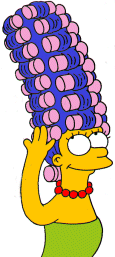
\includegraphics[width=\textwidth]{marge001}
        \caption{Marge}
        \label{fig:marge}
    \end{subfigure}
    \caption{Exemplos de imagens}\label{fig:exemplos}
\end{figure}

Na Figura~\ref{fig:exemplos} são apresentados exemplos de imagens para cada uma das cinco classes.
Foram utilizados três métodos para extração de características: Histograma de cor, Momentos de Hu e Histograma da orientação dos gradientes {\it Histogram of oriented gradients} (HOG).
Inicialmente toda imagem recebida pelo módulo de extração é redimensionada para $150 \times 150$, em seguida é enviada para o método de extração de características selecionado.

\subsection{Extração de características}

Para o histograma de cor, cada canal (cor de 0 à 255) foi dividida em quatro partes (bins) e calculado quantos pixels se encaixam em cada parte (para cada cor). 
Retornando assim um vetor de características com 64 posições.
A quantidade de divisões (bins) é um parâmetro do método, porém apenas o valor quatro foi avaliado.
Outro método de extração de características utilizado foi o Momentos de Hu, que são invariantes a translação, rotação e escala.
Para sua utilização a imagem foi convertida para tons de cinza. Este método retorna um vetor de sete características (os sete momentos de Hu).
É sugerido que este método seja utilizado após a segmentação da imagem, porém esta etapa não foi realizada.
O terceiro método de extração de características utilizado foi o HOG, que utiliza os gradientes da imagem para capturar contornos, silhuetas e algumas informações de textura.

\subsection{Classificação}

Para a classificação das imagens, inicialmente os vetores de característica são normalizados.
Em seguida é aplicado um dos três classificadores implementados: {\it Linear DiscriMínimoant Analysis} (LDA), {\it K-th Nearest Neighbor} (KNN) e {\it Support Vector Machine } (SVM).
O método KNN, apresenta dois parâmetros, o número de vizinhos ($k$) e a métrica de distância.
Os valores utilizados foram $k=5$ e distância euclidiana. Não foram avaliados outros valores.
Para o SVM o modelo foi aprendido por meio de {\it GridSearch}.

\subsection {Fusão}

Para a fusão foram construídas duas lista, uma com os métodos de extração de características ({\it features}) e outra com os classificadores ({\it clasifiers}).
Então para cada combinação $[feature, Classificador]$ é construído e treinado um classificador.
Em seguida os exemplos de teste são classificados utilizando todos os classificadores construídos.
Para a fusão da saída dos classificadores foram implementados cinco métodos: soma, mínimo, máximo, produto e {\it Borda count}.
Os quatro primeiros utilizam as probabilidades retornadas por cada classificador, 
enquanto para o {\it Borda count} foi calculado os rankings (a partir das probabilidades).

\section {Análise da classificação}

Inicialmente foram avaliados todas as combinações de métodos de extração de características e de classificação.
Assim, foram instanciados nove classificadores e os resultados foram agrupados por método de extração de características.
Os resultados são apresentados nas Tabelas \ref{tbl:colorhistogram}, \ref{tbl:hog} e \ref{tbl:humoments}.
A escolha dos métodos de extração de características apresentaram um maior impacto no acerto do que os métodos de classificação.
Além disso, todos os métodos apresentaram {\it bias} para o personagem \texttt{bart}, provavelmente por ser a classe que apresenta o maior número de exemplos (tanto no teste quanto na validação).

Para análise do desempenho dos classificadores é apresentado o acerto geral, o acerto para cada classe e também o acerto médio nas cinco classes.
Esta análise permite identificar classificadores que tenham um bom desempenho geral, porém tendem a acertar uma (ou poucas) classes (as que tenham mais exemplos).
Por exemplo, a combinação Histograma de cor e SVM apresentou melhor desempenho geral e pior desempenho médio do que a combinação Histograma de cor e KNN.

\begin{table}[!htb]
\centering
\caption{Matrizes de confusão para os classificadores utilizando Histograma de Cor}
\label{tbl:colorhistogram}
\small
\singlespacing
\begin{tabular}{l|l|l|l|l|l|l}
\hline
\multicolumn{7}{l}{\textbf{Classificador: SVM}}                                                \\ \hline
\multicolumn{7}{l}{\textbf{Acerto: 62.11\%}}                                                  \\ \hline
          & bart      & homer     & lisa      & maggie    & marge          & Acerto:            \\ \hline
bart      & 27        & 7         & 1         & 0         & 0              & 77.14\%          \\ \hline
homer     & 5         & 15        & 3         & 1         & 1              & 60.00\%          \\ \hline
lisa      & 4         & 3         & 6         & 0         & 0              & 46.15\%          \\ \hline
maggie    & 1         & 3         & 0         & 8         & 0              & 66.67\%          \\ \hline
marge     & 5         & 1         & 1         & 0         & 3              & 30.00\%          \\ \hline
          &           &           & \textbf{} & \textbf{} & \textbf{media} & \textbf{55.99\%} \\ \hline
\multicolumn{7}{l}{\textbf{Classificador: LDA}}                                                \\ \hline
\multicolumn{7}{l}{\textbf{Acerto: 68.42\%}}                                                  \\ \hline
          & bart      & homer     & lisa      & maggie    & marge          & Acerto:            \\ \hline
bart      & 30        & 4         & 1         & 0         & 0              & 85.71\%          \\ \hline
homer     & 2         & 16        & 6         & 0         & 1              & 64.00\%          \\ \hline
lisa      & 2         & 3         & 8         & 0         & 0              & 61.54\%          \\ \hline
maggie    & 2         & 2         & 0         & 8         & 0              & 66.67\%          \\ \hline
marge     & 3         & 1         & 3         & 0         & 3              & 30.00\%          \\ \hline
          &           &           &           &           & \textbf{media} & \textbf{61.58\%} \\ \hline
\multicolumn{7}{l}{\textbf{Classificador: KNN}}                                                \\ \hline
\multicolumn{7}{l}{\textbf{Acerto: 65.26\%}}                                                  \\ \hline
          & bart      & homer     & lisa      & maggie    & marge          & Acerto:            \\ \hline
bart      & 32        & 2         & 1         & 0         & 0              & 91.43\%          \\ \hline
homer     & 7         & 12        & 5         & 1         & 0              & 48.00\%          \\ \hline
lisa      & 3         & 1         & 8         & 1         & 0              & 61.54\%          \\ \hline
maggie    & 4         & 1         & 0         & 7         & 0              & 58.33\%          \\ \hline
marge     & 7         & 0         & 0         & 0         & 3              & 30.00\%          \\ \hline
          &           &           &           & \textbf{} & \textbf{media} & \textbf{57.86\%} \\ \hline
\end{tabular}
\end{table}

O método Histograma de cor (Tabela~\ref{tbl:colorhistogram}) apresentou melhores resultados do que os demais métodos de extração de características.
Tanto em termos de acerto geral, quanto em termos de acerto médio entre as cinco classes.
A escolha do método de classificação apresentou menor impacto no desempenho, com pequena vantagem para o LDA (no caso de Histograma de cor).

\begin{table}[!htb]
\centering
\caption{Matrizes de confusão para os classificadores utilizando Histograma de orientação dos gradientes}
\label{tbl:hog}
\small
\singlespacing
\begin{tabular}{l|l|l|l|l|l|l} \hline
\multicolumn{7}{l}{\textbf{Classificador: SVM}}                                                \\ \hline
\multicolumn{7}{l}{\textbf{Acerto: 43.16\%}}                                                  \\ \hline
          & bart      & homer     & lisa      & maggie    & marge          & Acerto:            \\ \hline
bart      & 26        & 9         & 0         & 0         & 0              & 74.29\%          \\ \hline
homer     & 14        & 9         & 1         & 0         & 1              & 36.00\%          \\ \hline
lisa      & 5         & 5         & 3         & 0         & 0              & 23.08\%          \\ \hline
maggie    & 3         & 5         & 1         & 2         & 1              & 16.67\%          \\ \hline
marge     & 5         & 3         & 1         & 0         & 1              & 10.00\%          \\ \hline
          &           &           &           &           & \textbf{media} & \textbf{32.01\%} \\ \hline
\multicolumn{7}{l}{\textbf{Classificador: LDA}}                                                \\ \hline
\multicolumn{7}{l}{\textbf{Acerto: 43.16\%}}                                                  \\ \hline
          & bart      & homer     & lisa      & maggie    & marge          & Acerto:            \\ \hline
bart      & 26        & 6         & 2         & 1         & 0              & 74.29\%          \\ \hline
homer     & 11        & 9         & 0         & 2         & 3              & 36.00\%          \\ \hline
lisa      & 9         & 3         & 1         & 0         & 0              & 7.69\%           \\ \hline
maggie    & 6         & 2         & 0         & 4         & 0              & 33.33\%          \\ \hline
marge     & 6         & 2         & 1         & 0         & 1              & 10.00\%          \\ \hline
          &           &           &           &           & \textbf{media} & \textbf{32.26\%} \\ \hline
\multicolumn{7}{l}{\textbf{Classificador: KNN}}                                                \\ \hline
\multicolumn{7}{l}{\textbf{Acerto: 49.47\%}}                                                  \\ \hline
          & bart      & homer     & lisa      & maggie    & marge          & Acerto:            \\ \hline
bart      & 32        & 3         & 0         & 0         & 0              & 91.43\%          \\ \hline
homer     & 11        & 14        & 0         & 0         & 0              & 56.00\%          \\ \hline
lisa      & 8         & 4         & 1         & 0         & 0              & 7.69\%           \\ \hline
maggie    & 9         & 3         & 0         & 0         & 0              & 0.00\%           \\ \hline
marge     & 7         & 3         & 0         & 0         & 0              & 0.00\%           \\ \hline
          &           &           &           &           & \textbf{media} & \textbf{31.02\%} \\ \hline
\multicolumn{7}{l}{\multirow{2}{*}{}}                                                       \\
\end{tabular}
\end{table}

\begin{table}[!htb]
\centering
\caption{Matrizes de confusão para os classificadores utilizando Momentos de Hu}
\label{tbl:humoments}
\small
\singlespacing
\begin{tabular}{l|l|l|l|l|l|l} \hline
\multicolumn{7}{l}{\textbf{Classificador: SVM}}                                                \\ \hline
\multicolumn{7}{l}{\textbf{Acerto: 44.21\%}}                                                  \\ \hline
          & bart      & homer     & lisa      & maggie    & marge          & Acerto:            \\ \hline
bart      & 28        & 7         & 0         & 0         & 0              & 80.00\%          \\ \hline
homer     & 14        & 9         & 0         & 2         & 0              & 36.00\%          \\ \hline
lisa      & 11        & 2         & 0         & 0         & 0              & 0.00\%           \\ \hline
maggie    & 8         & 3         & 0         & 0         & 1              & 0.00\%           \\ \hline
marge     & 3         & 2         & 0         & 0         & 5              & 50.00\%          \\ \hline
\textbf{} & \textbf{} & \textbf{} & \textbf{} & \textbf{} & \textbf{media} & \textbf{33.20\%} \\ \hline
\multicolumn{7}{l}{\textbf{Classificador: LDA}}                                                \\ \hline
\multicolumn{7}{l}{\textbf{Acerto: 41.05\%}}                                                  \\ \hline
          & bart      & homer     & lisa      & maggie    & marge          & Acerto:            \\ \hline
bart      & 25        & 6         & 0         & 1         & 3              & 71.43\%          \\ \hline
homer     & 15        & 7         & 0         & 3         & 0              & 28.00\%          \\ \hline
lisa      & 11        & 1         & 0         & 0         & 1              & 0.00\%           \\ \hline
maggie    & 8         & 1         & 0         & 1         & 2              & 8.33\%           \\ \hline
marge     & 3         & 1         & 0         & 0         & 6              & 60.00\%          \\ \hline
\textbf{} & \textbf{} & \textbf{} & \textbf{} & \textbf{} & \textbf{media} & \textbf{33.55\%} \\ \hline
\multicolumn{7}{l}{\textbf{Classificador: KNN}}                                                \\ \hline
\multicolumn{7}{l}{\textbf{Acerto: 37.89\%}}                                                  \\ \hline
          & bart      & homer     & lisa      & maggie    & marge          & Acerto:            \\ \hline
bart      & 20        & 6         & 6         & 1         & 2              & 57.14\%          \\ \hline
homer     & 10        & 8         & 3         & 3         & 1              & 32.00\%          \\ \hline
lisa      & 10        & 0         & 0         & 2         & 1              & 0.00\%           \\ \hline
maggie    & 4         & 2         & 1         & 3         & 2              & 25.00\%          \\ \hline
marge     & 2         & 1         & 1         & 1         & 5              & 50.00\%          \\ \hline
\textbf{} & \textbf{} & \textbf{} & \textbf{} & \textbf{} & \textbf{media} & \textbf{32.83\%} \\ \hline
\end{tabular}
\end{table}

Nos experimentos realizados com Histograma de orientação dos gradientes (HOG) (Tabela~\ref{tbl:hog}) o desempenho foi relativamente mais baixo ($49.47\%$ no melhor caso [KNN]).
Principalmente em termos de desempenho médio. 
Neste caso a diferença entre o acerto para uma classe e outra chega a ser de $91.43\%$ (KNN).
Sendo que, em geral, poucos exemplos foram classificados nas duas últimas classes (as que apresentam menos exemplos).

Utilizando o método de extração de características Momentos de Hu (Tabela~\ref{tbl:humoments}) o desempenho geral também foi ruim.
Porém, nos três casos (SVM, LDA e KNN) apresentou melhor desempenho médio do que quando utilizado HOG.

\begin{table}[!htb]
\centering
\caption{Fusão dos nove métodos de classificação instanciados}
\label{tbl:fusionall}
\small
\singlespacing
\begin{tabular}{l|l|l|l|l|l|l}
\hline
\multicolumn{7}{l}{\textbf{Borda}}                                                          \\ \hline
\multicolumn{7}{l}{\textbf{Acerto:: 53.68\%}}                                                 \\ \hline
          & bart      & homer     & lisa      & maggie    & marge          & Acerto:            \\ \hline
bart      & 34        & 1         & 0         & 0         & 0              & 97.14\%          \\ \hline
homer     & 13        & 12        & 0         & 0         & 0              & 48.00\%          \\ \hline
lisa      & 11        & 1         & 1         & 0         & 0              & 7.69\%           \\ \hline
maggie    & 7         & 3         & 0         & 2         & 0              & 16.67\%          \\ \hline
marge     & 8         & 0         & 0         & 0         & 2              & 20.00\%          \\ \hline
\textbf{} & \textbf{} & \textbf{} & \textbf{} & \textbf{} & \textbf{media} & \textbf{37.90\%} \\ \hline
\multicolumn{7}{l}{\textbf{Soma}}                                                            \\ \hline
\multicolumn{7}{l}{\textbf{Acerto:: 67.37\%}}                                                 \\ \hline
          & bart      & homer     & lisa      & maggie    & marge          & Acerto:            \\ \hline
bart      & 33        & 2         & 0         & 0         & 0              & 94.29\%          \\ \hline
homer     & 7         & 17        & 1         & 0         & 0              & 68.00\%          \\ \hline
lisa      & 8         & 3         & 2         & 0         & 0              & 15.38\%          \\ \hline
maggie    & 2         & 2         & 0         & 8         & 0              & 66.67\%          \\ \hline
marge     & 4         & 1         & 1         & 0         & 4              & 40.00\%          \\ \hline
\textbf{} & \textbf{} & \textbf{} & \textbf{} & \textbf{} & \textbf{media} & \textbf{56.87\%} \\ \hline
\multicolumn{7}{l}{\textbf{Máximo}}                                                            \\ \hline
\multicolumn{7}{l}{\textbf{Acerto:: 63.16\%}}                                                 \\ \hline
          & bart      & homer     & lisa      & maggie    & marge          & Acerto:            \\ \hline
bart      & 29        & 3         & 2         & 1         & 0              & 82.86\%          \\ \hline
homer     & 6         & 12        & 6         & 0         & 1              & 48.00\%          \\ \hline
lisa      & 3         & 3         & 7         & 0         & 0              & 53.85\%          \\ \hline
maggie    & 2         & 2         & 0         & 8         & 0              & 66.67\%          \\ \hline
marge     & 3         & 1         & 2         & 0         & 4              & 40.00\%          \\ \hline
\textbf{} & \textbf{} & \textbf{} & \textbf{} & \textbf{} & \textbf{media} & \textbf{58.27\%} \\ \hline
\multicolumn{7}{l}{\textbf{Mínimo}}                                                            \\ \hline
\multicolumn{7}{l}{\textbf{Acerto:: 47.37\%}}                                                 \\ \hline
          & bart      & homer     & lisa      & maggie    & marge          & Acerto:            \\ \hline
bart      & 31        & 3         & 0         & 1         & 0              & 88.57\%          \\ \hline
homer     & 14        & 11        & 0         & 0         & 0              & 44.00\%          \\ \hline
lisa      & 12        & 1         & 0         & 0         & 0              & 0.00\%           \\ \hline
maggie    & 7         & 1         & 1         & 3         & 0              & 25.00\%          \\ \hline
marge     & 9         & 1         & 0         & 0         & 0              & 0.00\%           \\ \hline
\textbf{} & \textbf{} & \textbf{} & \textbf{} & \textbf{} & \textbf{media} & \textbf{31.51\%} \\ \hline
\multicolumn{7}{l}{\textbf{Produto}}                                                        \\ \hline
\multicolumn{7}{l}{\textbf{Acerto:: 47.37\%}}                                                 \\ \hline
          & bart      & homer     & lisa      & maggie    & marge          & Acerto:            \\ \hline
bart      & 32        & 3         & 0         & 0         & 0              & 91.43\%          \\ \hline
homer     & 15        & 10        & 0         & 0         & 0              & 40.00\%          \\ \hline
lisa      & 12        & 1         & 0         & 0         & 0              & 0.00\%           \\ \hline
maggie    & 7         & 1         & 1         & 3         & 0              & 25.00\%          \\ \hline
marge     & 9         & 1         & 0         & 0         & 0              & 0.00\%           \\ \hline
\textbf{} & \textbf{} & \textbf{} & \textbf{} & \textbf{} & \textbf{media} & \textbf{31.29\%} \\ \hline
\end{tabular}
\end{table}

Foi avaliada a fusão dos nove classificadores (três métodos de extração de características combinados com três métodos de classificação) com cinco diferentes métodos de fusão.
Os métodos de fusão mais rígidos, (produto e mínimo) foram os que apresentaram o pior desempenho, principalmente quanto ao desempenho médio entre as cinco classes. Sendo pior do que a maioria dos nove classificadores aplicados individualmente.
O método {\it Borda count} apresentou um desempenho mediano porém pior do que todos os classificadores baseados em histograma de cor individualmente.
O método Máximo e Soma apresentaram desempenho mais próximo aos melhores aplicados individualmente.
Porém, ainda assim, menores do que o classificador LDA com Histograma de cor aplicado individualmente.
Este classificador obteve um desempenho de $68.42\%$ no geral e $61.58\%$ na média entre as classes.
Sendo que o melhor desempenho geral obtido por meio de fusão de classificadores foi com o método soma ($67.37\%$) e o melhor desempenho médio pelo método Máximo ($58.27\%$).

\begin{table}[!htb]
\centering
\caption{Fusão dos classificadores utilizando apenas Momentos de Hu e Histograma de cor}
\label{tbl:huandcolor}
\small
\singlespacing
\begin{tabular}{l|l|l|l|l|l|l}
\hline
\multicolumn{7}{l}{\textbf{Borda}}                                                          \\ \hline
\multicolumn{7}{l}{\textbf{Acerto: 54.74\%}}                                                  \\ \hline
          & bart      & homer     & lisa      & maggie    & marge          & Acerto:            \\ \hline
bart      & 32        & 2         & 1         & 0         & 0              & 91.43\%          \\ \hline
homer     & 10        & 12        & 1         & 2         & 0              & 48.00\%          \\ \hline
lisa      & 13        & 0         & 0         & 0         & 0              & 0.00\%           \\ \hline
maggie    & 5         & 2         & 0         & 5         & 0              & 41.67\%          \\ \hline
marge     & 6         & 1         & 0         & 0         & 3              & 30.00\%          \\ \hline
\textbf{} & \textbf{} & \textbf{} & \textbf{} & \textbf{} & \textbf{media} & \textbf{42.22\%} \\ \hline
\multicolumn{7}{l}{\textbf{Soma}}                                                            \\ \hline
\multicolumn{7}{l}{\textbf{Acerto: 67.37\%}}                                                  \\ \hline
          & bart      & homer     & lisa      & maggie    & marge          & Acerto:            \\ \hline
bart      & 31        & 3         & 1         & 0         & 0              & 88.57\%          \\ \hline
homer     & 5         & 14        & 4         & 1         & 1              & 56.00\%          \\ \hline
lisa      & 4         & 2         & 7         & 0         & 0              & 53.85\%          \\ \hline
maggie    & 2         & 2         & 0         & 8         & 0              & 66.67\%          \\ \hline
marge     & 4         & 1         & 1         & 0         & 4              & 40.00\%          \\ \hline
\textbf{} & \textbf{} & \textbf{} & \textbf{} & \textbf{} & \textbf{media} & \textbf{61.02\%} \\ \hline
\multicolumn{7}{l}{\textbf{Máximo}}                                                            \\ \hline
\multicolumn{7}{l}{\textbf{Acerto: 68.42\%}}                                                  \\ \hline
          & bart      & homer     & lisa      & maggie    & marge          & Acerto:            \\ \hline
bart      & 30        & 4         & 1         & 0         & 0              & 85.71\%          \\ \hline
homer     & 3         & 15        & 6         & 0         & 1              & 60.00\%          \\ \hline
lisa      & 2         & 3         & 8         & 0         & 0              & 61.54\%          \\ \hline
maggie    & 2         & 2         & 0         & 8         & 0              & 66.67\%          \\ \hline
marge     & 3         & 1         & 2         & 0         & 4              & 40.00\%          \\ \hline
\textbf{} & \textbf{} & \textbf{} & \textbf{} & \textbf{} & \textbf{media} & \textbf{62.78\%} \\ \hline
\multicolumn{7}{l}{\textbf{Mínimo}}                                                            \\ \hline
\multicolumn{7}{l}{\textbf{Acerto: 52.63\%}}                                                  \\ \hline
          & bart      & homer     & lisa      & maggie    & marge          & Acerto:            \\ \hline
bart      & 27        & 5         & 2         & 1         & 0              & 77.14\%          \\ \hline
homer     & 9         & 12        & 3         & 1         & 0              & 48.00\%          \\ \hline
lisa      & 11        & 1         & 1         & 0         & 0              & 7.69\%           \\ \hline
maggie    & 4         & 1         & 0         & 7         & 0              & 58.33\%          \\ \hline
marge     & 6         & 1         & 0         & 0         & 3              & 30.00\%          \\ \hline
\textbf{} & \textbf{} & \textbf{} & \textbf{} & \textbf{} & \textbf{media} & \textbf{44.23\%} \\ \hline
\multicolumn{7}{l}{\textbf{Produto}}                                                        \\ \hline
\multicolumn{7}{l}{\textbf{Acerto: 52.63\%}}                                                  \\ \hline
          & bart      & homer     & lisa      & maggie    & marge          & Acerto:            \\ \hline
bart      & 28        & 4         & 2         & 1         & 0              & 80.00\%          \\ \hline
homer     & 9         & 11        & 3         & 2         & 0              & 44.00\%          \\ \hline
lisa      & 11        & 1         & 1         & 0         & 0              & 7.69\%           \\ \hline
maggie    & 4         & 1         & 0         & 7         & 0              & 58.33\%          \\ \hline
marge     & 6         & 1         & 0         & 0         & 3              & 30.00\%          \\ \hline
\textbf{} & \textbf{} & \textbf{} & \textbf{} & \textbf{} & \textbf{media} & \textbf{44.01\%} \\ \hline
\end{tabular}
\end{table}

Visando melhorar o desempenho da fusão dos classificadores foi realizado um experimento sem o método de extração de características mais fraco (em termos de desempenho médio): Histograma da orientação do gradiente.
Foi observado que o desempenho geral e médio melhorou em todos os casos (exceto o desempenho geral da soma que manteve o mesmo valor).
Ainda, em relação ao desempenho geral, o método Máximo ultrapassou o da Soma, e alcançou o valor do classificador LDA com Histograma de cor.
Sendo, o método Máximo conseguiu o melhor valor de desempenho médio até agora ($62.78\%$).

\section{Conclusões}

Neste trabalho foram comparados três métodos de extração de características e três métodos de classificação para a base de dados SIMPSONS.
Também foram avaliados cinco métodos de fusão de classificadores e a influência dos classificadores utilizados na qualidade da fusão.
A qualidade dos métodos de extração de características na base de imagens foi crucial para o desempenho dos classificadores, sendo que o método de Histograma de cor foi o método com melhor desempenho.
Entre os métodos de classificação (KNN, LDA e SVM) o desempenho pode ser considerado equivalente ou próximo.
A fusão dos classificadores não conseguiu sobrepor o baixo desempenho dos classificadores fracos, que resultaram em um desempenho inferior dos métodos de fusão do que o LDA com histograma de cor aplicado individualmente.
Buscando suprir esta dificuldade foi realizada uma análise sem o método de extração de característica mais fraco.
O resultado geral da fusão foi equivalente ao melhor individualmente porém o desempenho médio foi $1.20\%$ melhor.

O sistema implementado apresenta como pontos fracos os métodos de extração de características, que não discriminam as classes do problema, sendo que poderiam ter sido utilizados métodos de extração de características melhor discriminantes.
Além disso a base de imagens utilizada apresenta poucas imagens de algumas classes, o que dificulta o aprendizado.
Para isso, poderia ter sido aplicadas técnicas pra aumentar a quantidade de exemplos na base, aplicando alterações nas imagens existentes.
Os parâmetros dos métodos poderiam ter sido melhor configurados, utilizando técnicas automáticas de configuração de parâmetros, por exemplo {\it Iterated racing}. Ou ainda algoritmos evolutivos multi-objetivo, considerando como objetivos conflitantes a taxa de classificação em cada classe.
Como pontos fortes do sistema é possível citar a taxa de acerto com histograma de cor.
É possível citar ainda a forma com que foram avaliados os classificadores, considerando o desempenho médio por classe, o que ameniza o desempenho de classificadores tendenciosos.
É sugerido ainda a comparação com Redes Neurais Convolucionais que pode apresentar um bom desempenho na classificação de imagens.

\end{document}


